\documentclass[11pt, a4paper]{article}

\usepackage[utf8]{inputenc}
\usepackage[T1]{fontenc}
\usepackage[english]{babel}
\usepackage{hyperref}
\usepackage{framed}
\usepackage{geometry}
\usepackage{tikz}
\usetikzlibrary{arrows,shapes,snakes,positioning}
\usepackage{lscape}
\usepackage{csquotes}
\usepackage{todonotes}
\usepackage{color}

\title{LINGI2251: Assignment 1}
\author{Florian Thuin and Nicolas Houtain}
\date{\today}

\begin{document}
\maketitle
\tableofcontents

\section{Requirements}
\subsection{Requirement issues and adopted corrections}

\paragraph{Requirement 1} After the purchase of gasoline, the gas pump
reports the number of gallons purchased to the GSCS.\@ The GSCS updates the
remaining inventory.

\paragraph{Requirement 2} After the purchase of gasoline, the gas pump
reports the dollar amount of the purchase to the GSCS.\@ The maximum value of
a purchase is $\$~999.99$. The GSCS then causes the gas pump interface to
query the customer as to payment type.

\begin{framed}
    \paragraph{Critics}
    \begin{itemize}
        \item Requirement 1 and 2 are strongly connected because the
            amount of dollars depends on the number of gallons.

            In this way, we think that it should only be one
            requirement instead of two.

        \item \enquote{After} is a infinite length of time and must be more
            precise such as \enquote{Immediatly after}.
    \end{itemize}

    \paragraph{Requirement 1 and 2 corrected} Immediatly after the purchase of
    gasoline, the gas pump reports the number of gallons purchased and the
    amount of dollars of the purchase to the GSCS.\@ The maximum value of
    a purchase is $\$999.99$.
    When the GSCS receives the report, he updates the remaining
    inventory and causes the gas pump interface to query the customer as to
    payment type.
\end{framed}

\paragraph{Requirement 3} The customer may choose to be billed at the time
of purchase, or to be sent a monthly bill. If billing is to be done at time
of purchase, the gas pump interface queries the customer as to whether
payment will be made by cash or credit card. If the purchase is to be placed
on a monthly bill, the gas pump interface instructs the customer to see the
cashier. If an invalid or no response is received, the GSCS bills at the
time of purchase.

\begin{framed}
    \paragraph{Critics}
    \begin{itemize}
        \item There should be a time limit to says that there is no
            response.
        \item It's not explicit that the customer choose how to pays
            through gas pump interface.
    \end{itemize}

    \paragraph{Requirement 3 corrected} When the gas pump interface queries the
    customer as to payment type, he may choose to be billed at the
    time of purchase, or to be sent a monthly bill.
    If billing is to be done at time of purchase, the gas pump
    interface queries the customer as to whether payment will be
    made by cash or credit card. If the purchase is to be placed on
    a monthly bill, the gas pump interface instructs the customer to
    see the cashier. If an invalid response is received or there is
    no response during one minute, the GSCS bills at the time of purchase.
\end{framed}

\paragraph{Requirement 4} If the customer has selected to pay at the time of
purchase, he or she can choose to pay by cash or credit card. If the
customer selects cash, the gas pump interface instructs the customer to see
the cashier. If the customer selects credit card, the gas pump interface
instructs the customer to swipe his or her credit card through the credit
card reader. If an invalid or no selection is made, the GSCS will default
to credit card payment.

\begin{framed}
    \paragraph{Critics}
    \begin{itemize}
        \item There should be a time limit to says that there is no
            response.
    \end{itemize}

    \paragraph{Requirement 4 corrected} If the customer has selected to pay at the time of
    purchase, he or she can choose to pay by cash or credit card. If the
    customer selects cash, the gas pump interface instructs the customer to see
    the cashier. If the customer selects credit card, the gas pump interface
    instructs the customer to swipe his or her credit card through the credit
    card reader. If an invalid selection or no selection during one
    minute is made, the GSCS will default to credit card payment.
\end{framed}

\paragraph{Requirement 5} If payment is to be made by credit card, then the
card reader sends the credit card number to the GSCS.\@ If the GSCS receives
an invalid card number, then a message is sent to the gas pump interface
asking the customer to swipe the card through the card reader again. After
the account number is obtained, the account number and purchase price are
sent to the credit card system, and the GSCS and gas pump interface are
reset to their initial state. The purchase price sent can be up
to \${}10000.

\begin{framed}
    \paragraph{Critics}
    \begin{itemize}
        \item It's not complete because the requirement don't take into
            account that potentially the card reader is not able to read
            the card for some external reasons such as a invalid card or an
            issue with the card reader.
        \item It's not consistent to have a purchase price up to \$10000
            because the requirement 2 defines an upper bound to \$999.99.
        \item It's not consistent with the given definition of the credit card
            reader that says that it \enquote{reads the credit card number and
            sends it to the GSCS}. We will suppose that, as the GSCS already
            know the purchase price, the credit card reader sends only the
            credit card account number to the GSCS and the GSCS forwards the
            purchase amount and the credit card account number to the credit
            card system.
    \end{itemize}

    \paragraph{Requirement 5 corrected} If payment is to be made by credit card, then the
    card reader sends the credit card number to the GSCS.\@ If the GSCS receives
    an invalid card number, then a message is sent to the gas pump interface
    asking the customer to swipe the card through the card reader again.
    If after three times the account is not obtained, the gas pump
    interface instructs the customer to see the cashier.
    If the account number is obtained within the three times, the
    credit card account number is sent to the GSCS.\@ The GSCS then sends the
    credit card account number and the purchase price (up to \$999.99) to the
    credit card system and cause the gas pump interface to
    reset to its initial state.
\end{framed}

\paragraph{Requirement 6} The cashier is responsible for accepting the
customer's payment and making change, if necessary. When payment is
complete, the cashier indicates this on the cashier's interface. The GSCS
and the gas pump interface then return to the initial state.

\begin{framed}
    \paragraph{Critics}
    \begin{itemize}
        \item It is not stated how the cashier knows the amount for the payment.
        \item The cashier is responsible for accepting cash payment or
            monthly billing but not credit card payment.
        \item The GSCS should not return to its initial state just because one
        payment is completed, if there are multiple gas pumps for example, we
        don't want the GSCS to skip other actions.
    \end{itemize}

    \paragraph{Requirement 6 corrected} If the customer's choice is cash payment
    or monthly billing, the GSCS sends the purchase amount to the cashier's
    interface to display it for the cashier. The cashier is responsible for
    accepting monthly billing or the
    customer's cash payment and making change, if necessary. When payment is
    complete, the cashier indicates this on the cashier's interface that
    forwards it to the GSCS.\@ The gas
    pump interface then returns to the initial state.
\end{framed}

\paragraph{Requirement 7} If payment is to be made by monthly bill, the
purchase price is displayed on the cashier's interface. The cashier
selects an option from the cashier's interface, alerting the GSCS that the
payment will be placed on a monthly bill. The GSCS then prompts the cashier
to enter the billing account number.

\paragraph{Requirement 8} The customer must give the billing account number
to the cashier, who then enters it at the cashier's interface. If a valid
billing account number is entered, then the billing account number, purchase
price, and a brief description of the type of transaction is logged. If an
invalid billing account number is entered, an error message is displayed
and the cashier is prompted to enter it again. The cashier must also have
the option to cancel the operation, in which case the cashier's interface
reverts to showing the purchase price and the cashier can again either
receive cash or indicate that monthly billing should be used.

\begin{framed}
    \paragraph{Critics}
    \begin{itemize}
        \item There is no sens to have two different requirement mainly
            if the requirement 8 is more complete than the requirement
            7. Indeed, the requirement 7 don't take in account the
            case where the customer has no ability to perform a
            monthly billing.
        \item There is no miracle in the display of the purchase price on the
        cashier's interface, it should be stated that it is sends by the GSCS.\@
        \item \enquote{A brief description of the type of transaction} isn't
        well defined, but we can't really correct it here.
    \end{itemize}

    \paragraph{Requirement 7 and 8 corrected} If payment is to be made by monthly bill as
    chosen by the customer, the GSCS sends the
    purchase price to the cashier's interface that displays it to the cashier.
    The customer must give the billing account number
    to the cashier, who then enters it at the cashier's interface. If a valid
    billing account number is entered, then the GSCS logs the billing account number, purchase
    price, and a brief description of the type of transaction. If an
    invalid billing account number is entered, the GSCS sends an error message
    that will be displayed on the cashier's interface, causing the cashier to
    enter the cashier to enter the billing account number again. The cashier must also have
    the option to cancel the operation, in which case the cashier's interface
    reverts to showing the purchase price and the cashier can again either
    receive cash or indicate that monthly billing should be used.
\end{framed}

\paragraph{Requirement 9} To pay a monthly bill, the customer must send
the payment along with the billing account number. The cashier enters
monthly payments by first selecting the appropriate option from the
cashier's interface. The GSCS then sends a message to the cashier's
interface. The GSCS then sends a message to the cashier's interface
prompting the cashier to enter the billing account number, the amount
remitted, and the type of payment. If any of these pieces of information
are not entered or are invalid, payment cannot be processed; an error
message will be displayed, and the cashier's interface will be returned
to the previous screen. If the type of payment is credit card, the credit
card account number must also be entered, and then the paper credit card
receipt will be photocopied and stored with the rest of the year's receipts.

\begin{framed}
    \paragraph{Critics}
    \begin{itemize}
        \item It's ambiguous because we don't know how the customer send
            the payment. By mail or go to the gas pump? The definition of the
            cashier says it only accepts cash payment, there is no credit card
            related hardware inside the cashier's interface, we will assume he
            enters the billing account number along with the related information
            of payment inside the GSCS.\@

        \item \enquote{by selecting the appropriate option} is not precise
            enough because there is only one appropriate option in that case is
            \enquote{pay a monthly bill}.

        \item The fact that the receipt will be photocopied is
            completely irrelevant for the requirements of the system.
    \end{itemize}

    \paragraph{Requirement 9 corrected} To pay a monthly bill, the customer must send
    a cash payment along with the billing account number or the credit card account
    number along with the billing account number and the amount remitteed. The
    cashier selects the monthly payment option from the
    cashier's interface. The GSCS then sends a message to the cashier's interface
    prompting the cashier to enter the billing account number, the amount
    remitted, and the type of payment. If any of these pieces of information
    are not entered or are invalid, payment cannot be processed; an error
    message will be displayed, and the cashier's interface will be returned
    to the previous screen. If these pieces of informations are valid, then the
    transaction is logged in the GSCS.\@
\end{framed}

\paragraph{Requirement 10} Unless otherwise specified, if the GSCS receives
invalid input it will send an error message to the cashier's interface.
The cashier will be expected to take appropriate action, which may
involve shutting the system down for maintenance.

\begin{framed}
    \begin{itemize}
        \item This requirement shows that the system isn't well specified
        because it assumes that it doesn't handle every situation. If the GSCS
        is able to send an error message to the cashier's interface, it means
        that the system will handle the error in some way, which means that
        is could be possible to specify explicitly the error and maybe to
        handle it otherwise.
        \item There is another problem: the cashier's definition doesnt' involve
        shutting down the system, if he can do that it should be stated that he
        can also start the system.
    \end{itemize}

    \paragraph{Requirement 10 corrected} Unless otherwise specified, if the GSCS
    receives an invalid input, it will send an error message to the cashier's
    interface. The cashier will be expected to take appropriate action, which
    may involve system maintenance.
\end{framed}

\paragraph{Non-functional requirement 1} The system must always respond to
customer input within 5 minutes.

\paragraph{Non-functional requirement 2} The system should be easy to
extend, so that if necessary another payment option (e.g.\ bankcard) can be
added with minimal effort.

\begin{framed}
    \paragraph{Critics}
    \begin{itemize}
        \item This requirement is really ambiguous because it use some
            ambiguous notions such as \enquote{easy} or \enquote{minimal}.

        \item There is a lot of other payment options such as bitcoin
            which are not relevant for this system.
    \end{itemize}
\paragraph{Non-functional requirement 2 corrected} Extensions such as adding
bankcard payment could be possible without modifying the existing structure of
the system.
\end{framed}

\subsection{Other remarks}

These requirements doesn't cover everything that the system does: for example,
there isn't a word about how a customer can register into the system to place
a monthly bill. As those information aren't essential for what is asked during
this assignment, we feel free to process as we feel (for example by saying that
the customer can register to the cashier).


\section{Interfaces}

\subsection{Credit card system}



\subsection{Credit card reader}


\subsection{Gas pump}


\subsection{Gas pump interface}


\subsection{Customer}


\subsection{Cashier}


\subsection{Cashier interface}



\section{State of the system}
In this section, we will briefly describe the parts of the state of the
system. \newline

The GSCS stores and maintain data about:

\begin{description}
    \item[The gas pump] The gas pump transmits the amount of gallons dispensed,
    the GSCS stores it and knows the corresponding price generated from
    each purchase along with the payment type.

    \item[The customers] The GSCS has a database of registered users
    (name:text, address:text, phone number:text, billing account number:text, current bill: positive float). It also knows the status
    of the current purchase (validated or not).
\end{description}



\section{Data-flow diagram}
% Defines a `datastore' shape for use in DFDs.  This inherits from a
% rectangle and only draws two horizontal lines.
\makeatletter
\pgfdeclareshape{datastore}{
  \inheritsavedanchors[from=rectangle]
  \inheritanchorborder[from=rectangle]
  \inheritanchor[from=rectangle]{center}
  \inheritanchor[from=rectangle]{base}
  \inheritanchor[from=rectangle]{north}
  \inheritanchor[from=rectangle]{north east}
  \inheritanchor[from=rectangle]{east}
  \inheritanchor[from=rectangle]{south east}
  \inheritanchor[from=rectangle]{south}
  \inheritanchor[from=rectangle]{south west}
  \inheritanchor[from=rectangle]{west}
  \inheritanchor[from=rectangle]{north west}
  \backgroundpath{
    %  store lower right in xa/ya and upper right in xb/yb
    \southwest \pgf@xa=\pgf@x \pgf@ya=\pgf@y
    \northeast \pgf@xb=\pgf@x \pgf@yb=\pgf@y
    \pgfpathmoveto{\pgfpoint{\pgf@xa}{\pgf@ya}}
    \pgfpathlineto{\pgfpoint{\pgf@xb}{\pgf@ya}}
    \pgfpathmoveto{\pgfpoint{\pgf@xa}{\pgf@yb}}
    \pgfpathlineto{\pgfpoint{\pgf@xb}{\pgf@yb}}
 }
}

\makeatother
\begin{landscape}
    \begin{figure}
 \begin{tikzpicture}[
  font=\sffamily,
  every matrix/.style={ampersand replacement=\&,column sep=0.5cm,row sep=0.5cm},
  source/.style={draw,thick,rounded corners,fill=red!20,inner sep=.3cm},
  process/.style={draw,thick,ellipse,fill=yellow!20},
  sink/.style={source,fill=blue!20},
  datastore/.style={draw,very thick,shape=datastore,inner sep=.3cm},
  dots/.style={gray,scale=2},
  from/.style={->,>=stealth',shorten >=1pt,semithick,font=\sffamily\tiny},
  to/.style={<-,>=stealth',shorten >=1pt,semithick,font=\sffamily\tiny},
  every node/.style={align=center, text width=1.2cm, scale=0.8, font=\sffamily\tiny},
  node distance = 2.5cm
  ]


  % GSCS
  \node[sink] (gscs) {GSCS};

  % Place central point around GSCS
  \def\aCCS {6cm} \def\rCCS {-10cm}
  \def\aCI  {-8cm} \def\rCI {-0cm}
  \def\aCCR {-1cm} \def\rCCR {7cm}
  \def\aCLI {1cm} \def\rCLI {13cm}
  \node[source]    (ccs)    [above right= \aCCS and \rCCS of gscs] {CCS};
  \node[source]    (ci)     [above right= \aCI and \rCI of gscs]   {CI};
  \node[source]    (ccr)    [above right= \aCCR and \rCCR of gscs] {CCR};
  \node[source]    (client) [above right= \aCLI and \rCLI of gscs] {Customer};

  % Place point dependant of central point
  \def\rGP  {3cm}
  \def\rGPI {7cm}
  \def\rCA  {8cm}
  \def\bINV {5.5cm}
  \def\bREG {1cm}
  \node[source]    (gp)     [right=\rGP of ccs]   {GP};
  \node[source]    (gpi)    [below right= 0.5cm and  \rGPI of gp] {GPI};
  \node[datastore] (inv)    [below = \bINV of ccs] {Inventory};
  \node[datastore] (reg)    [below = \bREG of inv] {Registers};
  \node[source]    (cash)   [right= \rCA of ci]   {Cashier};



  % CCS
  \node[process] (ccsPay) [below=of ccs] {Payment};
  \node[process] (ccsPayOk) [below right=1.5cm and 0.5cm of ccs]{Repayment};

  % Inventory
  \node[process] (invUpd) [right= 1cm of inv] {Update inventory};
  
  % Registers
  \node[process] (regUpd) [right= 1cm of reg] {CRUD};

  % GP
  \node[process] (gpInfo) [below=1cm of gp] {Send purchase info};

  % GPI
  \node[process] (gpiAsk) [below left=0.5cm and 4cm of gpi] {Ask payment type};
  \node[process] (gpiChoice) [below right=0.3cm and 0.3cm of gpiAsk] {Reply choice};
  \node[process] (gpiMsg) [below right =0.3cm and 0.3cm  of gpiChoice] {Send msg};
  \node[process] (gpiReset) [below right=0.3cm and 0.3cm  of gpiMsg] {Reset};



  % Client
  \node[process] (cliOption) [above right=3cm and -4.0cm of client] {Choose option};
  \node[process] (cliInst) [below left=0.3cm and 0.3cm of cliOption] {Display msg};
  \node[process] (cliType) [below left=0.3cm and 0.3cm of cliInst] {Ask payment type};

  \node[process] (cliPur) [above right=1cm and 1cm of cliOption] {Purchase gas};

  % CCR
  \node[process] (ccrSwipe) [above right=0.7cm and 1cm of ccr] {Swipe card};
  \node[process] (ccrSend) [above left= 0cm and 1.5cm of ccr] {Send \#card};
  \node[process] (ccrError) [below left=0cm and 1.5cm of ccr] {Send error};

  % Cashier
  \node[process] (cashMaint) [below =1.0cm of ccrError] {Do maintenance};

  \node[process] (cashInput) [left=of cash] {Input data};
  \node[process] (cashCancel) [above=0.5cm of cashInput] {Cancel operation};
  \node[process] (cashShut) [below=0.5cm of cashInput] {Shut down};
  \node[process] (cashInst) [below=0.5cm of cashShut] {Display info};

  \node[process] (cashChange) [above right=0.5cm and 3cm of cash] {Give change};
  \node[process] (cashReport) [above left=0.3cm and 0.3cm of cashChange] {Report monthly};
  \node[process] (cashCash) [above left= 0.3cm and 0.3cm of cashReport] {Pay purchase};
  \node[process] (cashMont) [above left= 0.3cm and 0.3cm of cashCash] {Pay monthly};
  \node[process] (cashReg) [above left= 0.3cm and 0.3cm of cashMont] {Register};

  % CI
  \node[process] (ciError) [left=7.5cm of ci]{Send error};
  \node[process] (ciShut)     [above right=0.2cm and 0.4cm of ciError] {Shutting down};
  \node[process] (ciInfo)     [above right=0.2cm and 0.4cm of ciShut]{Send info};
  \node[process] (ciInput)    [above right=0.2cm and 0.4cm of ciInfo]{Send input};
  \node[process] (ciCash)     [above right=0.2cm and 0.4cm of ciInput]{Complete purchase};
  \node[process] (ciReport)   [above right=0.2cm and 0.4cm of ciCash]{Report monthly};
  \node[process] (ciMonthly)  [above right=0.2cm and 0.4cm  of ciReport]{Pay monthly};
  \node[process] (ciVal)  [above right=0.2cm and 0.4cm  of ciMonthly]{Validate account};


  %DRAW

  % CCS
  \path[to] (ccs) edge node[midway, above] {raw events} (ccsPay) ;
  \path[from] (ccs) edge node[midway, above] {raw} (ccsPayOk);

  % GP
  \path[from] (gp) edge node[midway, above] {raw events} (gpInfo) ;
  \path[to] (gp) edge node[midway, above] {raw} (cliPur);

  % INV
  \path[to] (inv) edge node[midway, above] {raw} (invUpd);
  \path[to] (reg) edge node[midway, above] {raw} (regUpd);


  % GPI
  \path[to] (gpi)   edge node[midway, above] {raw} (gpiReset)
  edge node[midway, above] {raw} (gpiMsg)
  edge node[midway, above] {raw} (cliOption)
  edge node[midway, above] {raw} (gpiAsk);
  \path[from] (gpi) edge node[midway, above] {raw} (gpiChoice)
  edge node[midway, above] {raw} (cliType)
  edge node[midway, above] {raw} (cliInst);

  % CCR
  \path[to] (ccr)   edge node[midway, above] {raw} (ccrSwipe);
  \path[from] (ccr) edge node[midway, above] {raw} (ccrError)
  edge node[midway, above] {raw} (ccrSend);

  % CLI
  \path[to] (client)   edge node[midway, above] {raw} (cliType)
  edge node[midway, above] {raw} (cashChange)
  edge node[midway, above] {raw} (cliInst);

  \path[from] (client) edge node[midway, above] {raw} (ccrSwipe)
  edge node[midway, above] {raw} (cliPur)
  edge node[midway, above] {raw} (cliOption)
  edge node[midway, above] {raw} (cashReport) 
  edge node[midway, above] {raw} (cashCash) 
  edge node[midway, above] {raw} (cashMont) 
  edge node[midway, above] {raw} (cashReg);

  % CASH
  \path[to] (cash) edge node[midway, above] {raw} (cashReport) 
  edge node[midway, above] {raw} (cashCash) 
  edge node[midway, above] {raw} (cashMont) 
  edge node[midway, above] {raw} (cashInst)
  edge node[midway, above] {raw} (cashReg);

  \path[from] (cash) edge node[midway, above] {raw} (cashChange) 
  edge node[midway, above] {raw} (cashShut)
  edge node[midway, above] {raw} (cashCancel)
  edge node[midway, above] {raw} (cashInput)
  edge node[midway, above] {raw} (cashMaint) ;

  % CI
  \path[from] (ci) 
  edge node[midway, above] {raw} (cashInst)
  edge node[midway, above] {raw} (ciShut)   
 edge node[midway, above] {raw}  (ciInput)  
 edge node[midway, above] {raw}  (ciCash)   
 edge node[midway, above] {raw}  (ciReport) 
 edge node[midway, above] {raw}  (ciMonthly);


  \path[to] (ci) 
  edge node[midway, above] {raw} (cashShut)
  edge node[midway, above] {raw} (cashCancel)
  edge node[midway, above] {raw} (cashInput)
 edge node[midway, above] {raw}  (ciInfo) 
 edge node[midway, above] {raw}  (ciVal)  
 edge node[midway, above] {raw}  (ciError);

  % GSCS
  \path[from] (gscs)  edge node[midway, above] {raw events} (ccsPayOk)
  edge  node[midway, above] {raw events} (gpiAsk) 
  edge node[midway, above] {raw events} (gpiMsg) 
  edge node[midway, above] {raw events} (gpiReset)
  edge node[midway, above] {raw} (invUpd)
  edge node[midway, above] {raw} (regUpd)
 edge node[midway, above] {raw}  (ciInfo) 
 edge node[midway, above] {raw}  (ciVal)  
 edge node[midway, above] {raw}  (ciError);

  \path[to] (gscs) edge  node[midway, above] {raw} (ccsPay)
  edge node[midway, above] {raw} (gpInfo)
  edge node[midway, above] {raw} (gpiChoice)
  edge node[midway, above] {raw} (ccrSend)
  edge node[midway, above] {raw} (cashMaint) 
  edge node[midway, above] {raw} (ccrError)
 edge node[midway, above] {raw}  (ciInput)  
 edge node[midway, above] {raw}  (ciCash)   
 edge node[midway, above] {raw}  (ciReport) 
 edge node[midway, above] {raw}  (ciMonthly);



\end{tikzpicture}
\caption{Data-flow diagram}
\label{fig:data-flow}
\end{figure}
\end{landscape}



\section{Class diagram}


The class diagram is showing on fig~\ref{fig:class-diagram}

\begin{landscape}
\begin{figure}[!h]
\includegraphics[width=\linewidth]{drafts/class_diagram.png}
\caption{Class diagram}
\label{fig:class-diagram}
\end{figure}
\end{landscape}




\section{Sequence diagrams}
\subsection{A customer successfully purchases gas and charges it on
a monthly bill}

The sequence diagram is shown on figure~\ref{fig:seq-diagram1}

\begin{landscape}
    \begin{figure}[!ht]
        \centering
        \includegraphics[width=\linewidth]{drafts/sequence_1.png}
        \caption{A customer succesfully purchases gas and charges it on a
        monthly bill}
        \label{fig:seq-diagram1}
    \end{figure}
\end{landscape}

\subsection{A customer purchases gas and attempts to pay by credit
card but his card is refused. He then pays by cash to the cashier.}

The sequence diagram is shown on figure~\ref{fig:seq-diagram2}

\begin{landscape}
    \begin{figure}[!ht]
        \centering
        \includegraphics[width=\linewidth]{drafts/sequence_2.png}
        \caption{A customer purchases gas and attempts to pay by credit card but
        his card is refused. He then pays by cash to the cashier.}
        \label{fig:seq-diagram2}
    \end{figure}
\end{landscape}

\subsection{The cashier successfully processes a monthly payment by
credit card.}

The sequence diagram is shown on figure~\ref{fig:seq-diagram3}

\begin{landscape}
    \begin{figure}[!ht]
        \centering
        \includegraphics[width=\linewidth]{drafts/sequence_3.png}
        \caption{The cashier successfully processes a monthly payment by credit
        card.}
        \label{fig:seq-diagram3}
    \end{figure}
\end{landscape}



\section{State diagrams}

\subsection{Gas pump interface}

\begin{figure}[!h]
    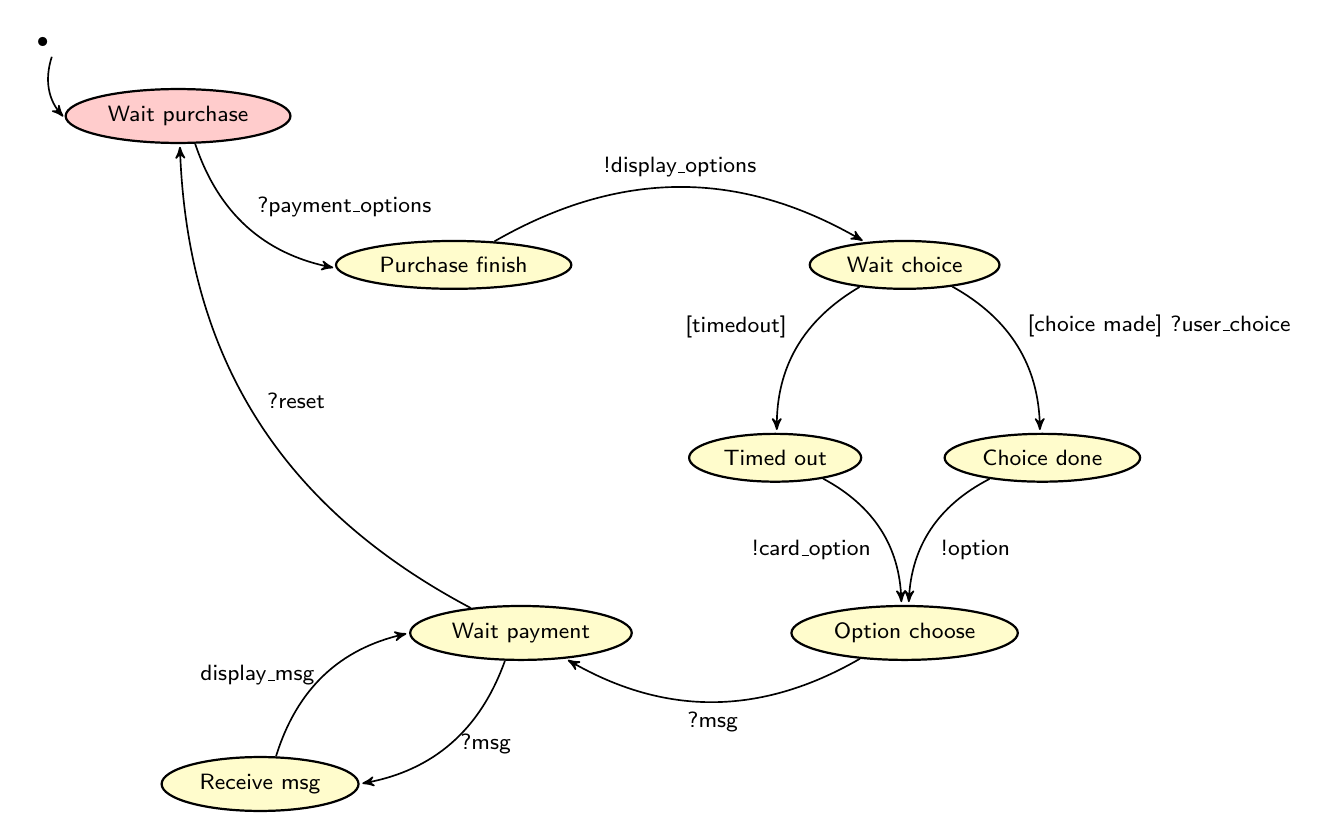
\begin{tikzpicture}[
            process/.style={draw,thick,ellipse,draw, minimum height=0.5cm, ellipse, fill=yellow!20},
            every node/.style={align=center, font=\sffamily\footnotesize},
            to/.style={->,>=stealth',shorten >=1pt,semithick,font=\sffamily\tiny},
            node distance = 2cm
  ]

  \node (start) {$\bullet$};
  \node[process, fill=red!20] (purchase) [below right=0.5cm and 0.5cm of start] {Wait purchase};
  \node[process] (finish) [below right=of purchase] {Purchase finish};
  \node[process] (display) [right=3cm of finish] {Wait choice};
  \node[process] (done) [below right=2cm and 0cm of display] {Choice done};
  \node[process] (timed) [below left=2cm and 0cm of display] {Timed out};
  \node[process] (choose) [below=4cm of display] {Option choose};
  \node[process] (paiment) [left=of choose] {Wait payment};
  \node[process] (msg) [below left=of paiment] {Receive msg};

  \draw[to] (purchase) edge[bend right] node[midway, above right] {?payment\_options} (finish);
  \draw[to] (finish) edge[bend left] node[midway, above] {!display\_options} (display);

  \draw[to] (display) edge[bend left] node[midway, above right] {[choice made] ?user\_choice} (done);
  \draw[to] (display) edge[bend right] node[midway, above left] {[timedout]} (timed);
  \draw[to] (done) edge[bend right] node[midway, below right] {!option} (choose);
  \draw[to] (timed) edge[bend left] node[midway, below left] {!card\_option} (choose);

  \draw[to] (choose) edge[bend left] node[midway, below] {?msg} (paiment);

  \draw[to] (paiment) edge[bend left] node[midway, right] {?msg} (msg);
  \draw[to] (msg) edge[bend left] node[midway, left] {display\_msg} (paiment);

  \draw[to] (paiment) edge[bend left] node[midway, above right] {?reset} (purchase);

  \draw[to] (start) edge[bend right] (purchase);


\end{tikzpicture}
\caption{State diagram of gas pump interface}
\label{fig:state-gpi}
\end{figure}

\subsection{Cashier interface}

\begin{figure}[!h]
    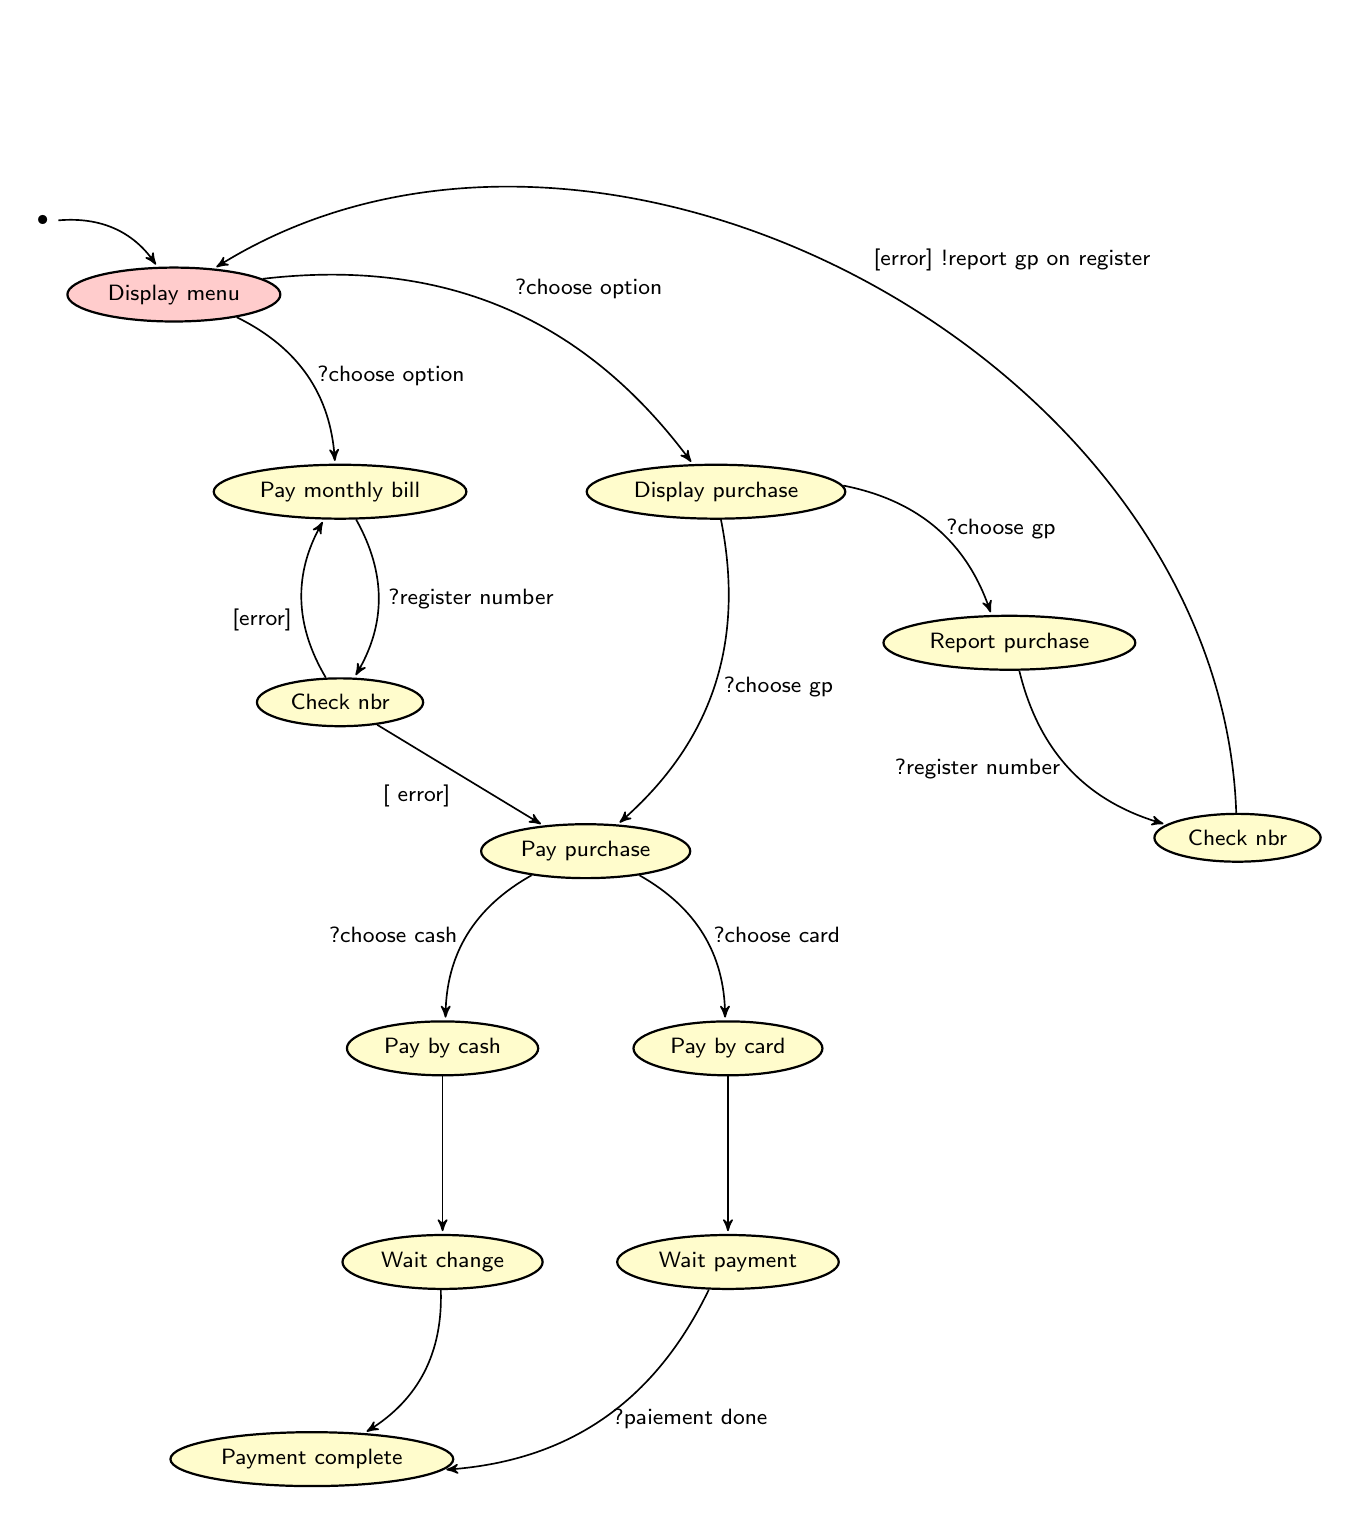
\begin{tikzpicture}[
            process/.style={draw,thick,ellipse,draw, minimum height=0.5cm, ellipse, fill=yellow!20},
            every node/.style={align=center, font=\sffamily\footnotesize},
            to/.style={->,>=stealth',shorten >=1pt,semithick,font=\sffamily\tiny},
            node distance = 2cm
  ]


  \node (start) {$\bullet$};
  \node[process, fill=red!20] (purchase) [below right=0.5cm and 0.5cm of start] {Display menu};

  \node[process] (monthly) [below right=2cm and 0cm of purchase] {Pay monthly bill};
  \node[process] (price) [right=1.5cm of monthly] {Display purchase};
  \node[process] (reg) [below= of monthly] {Check nbr};
  \node[process] (payment) [below right= of reg] {Pay purchase};

  \node[process] (report) [below right=of price] {Report purchase};
  \node[process] (check) [below right=2cm and 1cm of report] {Check nbr};

  \node[process] (card) [below right=2cm and 0cm of payment] {Pay by card};
  \node[process] (cash) [below left=2cm and 0cm of payment] {Pay by cash};
  \node[process] (wait) [below=of card] {Wait payment};
  \node[process] (change) [below=of cash] {Wait change};

  \node[process] (complete) [below left=2cm and 3cm of wait] {Payment complete};

  \draw[to] (start) edge[bend left] (purchase);

  \draw[to] (purchase) edge[bend left] node[above right] {?choose option} (price);
  \draw[to] (purchase) edge[bend left] node[right] {?choose option} (monthly);

  \draw[to] (monthly) edge[bend left] node[right] {?register number} (reg);

  \draw[to] (reg) edge[] node[below left] {[~error]} (payment);
  \draw[to] (reg) edge[bend left] node[below left] {[error]} (monthly);
  \draw[to] (price) edge[bend left] node[right] {?choose gp} (payment);

  \draw[to] (payment) edge[bend right] node[left] {?choose cash} (cash);
  \draw[to] (payment) edge[bend left] node[right] {?choose card} (card);
  
  \draw[to] (cash) edge[] node[left] {} (change);
  \draw[to] (card) edge[] node[right] {} (wait);

  \draw[to] (change) edge[bend left] node[left] {} (complete);
  \draw[to] (wait) edge[bend left] node[right] {?paiement done} (complete);

  \draw[to] (price) edge[bend left] node[right] {?choose gp} (report);
  \draw[to] (report) edge[bend right] node[left] {?register number}
  (check);
  \draw[to] (check) edge[bend right, in=-120, out=-60] node[above right] {[error] !report gp on register} (purchase);

\end{tikzpicture}
\caption{State diagram of cashier interface}
\label{fig:state-ci}
\end{figure}


\section{Conclusion}

In this assignment, we did our best to apply the theorical methods of
software development. We saw how important it was to have good
requirements to be able to build properly the rest of the structure of
the system. We also had to work iteratively because at first we missed
some methods or data needed and we had to add it while doing the next
diagrams. We limited our diagrams to our understanding of the
requirements, everything could be more complete and coherent if the
requirements were, but we had to work with partial information such that
everything might not seem clear from an external point-of-view.

\end{document}
